In this chapter, the details of approaches will be discussed. It starts with an overview of local interpretation methods and several variants of them are introduced respectively. Firstly, we present the binary feature flip idea which aims to characterize the impact of binary features by flipping the feature values. After that, we are interested in the effect of numeric features in the model by inspecting the outcome change of the model when the numeric feature values are perturbed to generate noises. Despite the "variable-specific" methods, we also focus on local interpretable model-agnostic explanations (LIME) which is able to explain individual predictions for any types of features and models. However, no theory can support why LIME can fit linear behavior locally on black box models. Therefore, we continue exploring Shapley value, which is a reasonable explanation method with well founded theory. In addition, the appealing approach assigns a contribution score for each feature value to smooth the path of interpreting the final prediction of individual instances by calculating the Shapley value. 

Then the following section describes the novel technique which combines the local interpretation methods and pattern mining technique. Since the target concept during subgroup discovery in our situation is either prediction change or feature influence score, therefore, the focus shall attribute to numeric target. Later, the standard approaches to measure the interestingness of subgroups are discussed. Furthermore, methods to avoid redundancy in subgroups are explored. 

%TO DO: provide more concrete examples
\section{Local interpretation methods}

In comparison to Global interpretable methods which are dedicated to explain the global model output by comprehending the entire datasets, it is more interesting to examine the model prediction for an individual instance. Besides, it could be observed that the global interpretation methods are less sensitive to noises if we make some perturbations on feature values, however, it could lead to tremendous changes in the prediction for an instance. Therefore, the local explanations shall preserve high accuracy than global explanations. In the following, few local interpretation methods will be covered in detail. 

\subsection{Binary feature value flip}

Binary feature implies that the feature only contains two unique values. In another words, if it is encoded as discrete numeric number, the feature value should be either 1 or 0. Thus, to flip binary feature value means to convert from 1 to 0 or the other way around. In practice, we could also use XOR operation to map from 1 to 0. For instance, gender is regarded as a binary feature which only holds value "male" and "female". 

As mentioned previously, the assumption is that we hold the dataset and the corresponding model trained on that dataset. Initially, we could obtain the prediction from the model for a specific instance. Then, a binary value is flipped on a chosen feature and afterwards a new prediction is generated by applying the model to the modified instance. Therefore, as a simple measurement, the effect of this binary feature could be estimated by the difference of two outputs. 

In practice, there are two variants to assess the variable influence. One way is to calculate the absolute difference of two predictions, and in this way we could ignore the bias of this binary feature on the original dataset. Literally to say, the binary feature is more influential when the difference becomes larger. In contrast, we could compute the difference for a defined direction, for example, we just care about the effect of gender changing from male to female. In this case, not only the magnitude of the effect is obtained, but also the positive or negative sign towards the prediction.  

\subsection{Numeric feature value perturbation}

As the name suggests, this technique is applicable on features whose type is numeric. The idea is that we could apply binary operations to the input values to produce new values, which serves as injecting noises into the original dataset. In particular, only addition and subtraction are considered in this situation. For example, an instance includes a numeric feature called "age" and we could perturb this feature value by increasing or decreasing by a certain value to obtain the modified value. 

The procedure of measuring the effect of a chosen input feature is similar to that in binary feature value flip approach. For classification or regression tasks, we could make predictions with the existing model on the instance we desire to explain. Afterwards, a new prediction is made on the adapted instance which is produced through perturbation on the selected numeric feature. And the impact of this numeric feature could be approximately evaluated by the absolute difference of two output predictions, which indicates that this particular feature plays an important role in this instance, causing unstable predictions. Roughly to say, larger prediction differences might imply the feature has stronger effect on the corresponding instance. 


\subsection{Local Surrogate: LIME}

Various criteria can be used to classify types for machine learning interpretability. Intrinsic interpretability, for example, is one type of the interpretability methods, which refers to models that are intrinsic interpretable owing to their simple structures, such as linear models or decision trees. In contrast, post hoc interpretability is meant to analyze the model interpretability after model training. As introduced earlier, permutation feature importance is a post hoc interpretation method. 
 
In this thesis, we would like to focus on post hoc interpretability, which indicates to explain model decisions after model has been trained. In particular, model agnostic interpretation methods, which extracts post hoc explanations by treating the original model as a black box, is highly valued. The model agnostic interpretation method is pretty flexible in terms of models, and it can work with any type of machine learning models, which provides a great advantage over model specific methods \cite{ribeiro2016model}. The principle behind is to learn an interpretable model on the decisions of the black box model and in return apply the interpretable model to those predictions that are expected to explain.  

Following this idea, it leads us to the local surrogate methods, which are able to explain individual predictions of any black box models in a faithful way. As a concrete implementation of local surrogate models, Local interpretable model-agnostic explanations (LIME) was initially proposed in paper \cite{ribeiro2016should}. 
%It might be noticed that the previously presented approaches are constrained within a certain situation and the stability or accuracy is not guaranteed either. Naturally, the aim comes to discover approaches to explain individual predictions of any black box models in a faithful way, leading us to the local surrogate methods. As a concrete implementation of local surrogate models, Local interpretable model-agnostic explanations (LIME) was initially proposed in paper \cite{ribeiro2016should}. 

The key point behind LIME is pretty straightforward. It is intended to explain individual explanations by fitting a simple interpretable model to locally approximate the underlying black box model. The typical choice of interpretable model could be regularized linear models like Lasso or decision trees. To elaborate more intuition for LIME, the toy example is shown in \ref{fig:lime}. This is a binary classification task and the regions colored with blue or pink are regarded as two distinct decisions. Evidently, this decision function can not be easily interpreted by a linear model. As a clarification, we are interested in the individual instance explanation, which is marked with bold red cross. In order to fit a local interpretable model, some artificial points are created by perturbing the original data point. The learned local model, marked by the dashed line, could in principle provide a faithful explanation for the target instance. 

\begin{figure}[H]% use[!htb] to force the latex ignore the defaut
	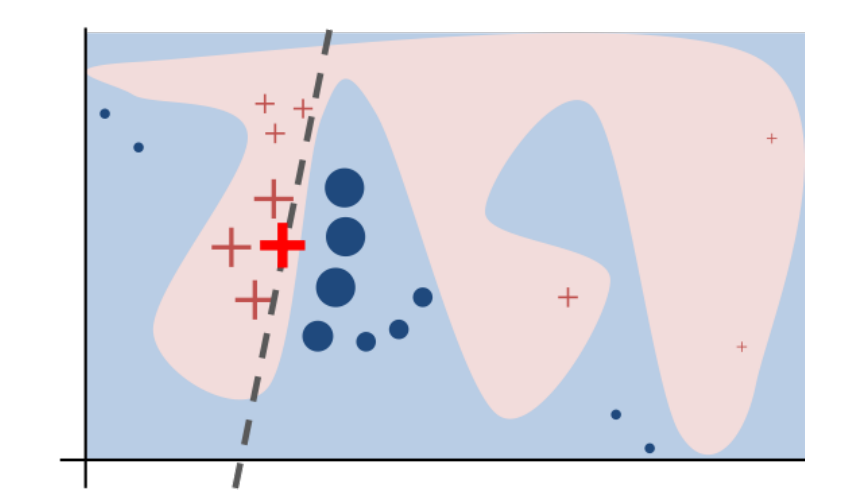
\includegraphics[width=0.9\textwidth]{imgs/lime.png}
	\caption{Binary classification task for a black box model. Decision regions are colored with blue or pink background. Instance to be explained are marked in bold red cross. Artificial points, marked as crosses and circles, are created by perturbing the instance of interest, whose size are weighted by the proximity to the instance. The dashed line expresses the fitted local interpretable model which could give faithful explanations.}
	\label{fig:lime}
\end{figure}

Apart from the intuition, we could argue for the faithfulness from mathematical perspective and the constraint of LIME could be represented as equation \ref{eq:lime}. 

\begin{equation} \label{eq:lime}
\begin{gathered}
\xi=\underset{g \in {G}}{\arg \min } L\left(f, g, \pi_{x}\right)+\Omega(g)
\end{gathered}
\end{equation}

As formally defined in equation, f is the black box model, g is the local explanation model needs to be figured out, and G is a group of interpretable models, which includes linear models, decision trees, or falling rule lists \cite{wang2015falling}. As depicted in figure, the weight is measured by the proximity of instance of interest to the surrounding artificial instances, which is defined as $\pi_{x}(z)$. And the complexity of explanation model g is described as $\Omega(g)$. For example, the complexity could be estimated by the depth of trees for decision trees models or by constraining the maximum number of features in linear models. Thus, as seen from the formula, in order to obtain the local explanation model for instance x, the loss L (e.g. mean squared error) should be minimized while maintaining the complexity as low as possible.

In practice, the general procedure to train a explanation model is described as follows: First, select an individual instance that we desire to explain for its black box prediction. Then, generate artificial data points by perturbing the selected sample and make predictions for these new instances using original model. Afterwards, calculate the weights for new instances according to their proximity to the instance being explained. Next, fit a weighted, interpretable model on the obtained dataset. Finally, interpret the instance prediction by utilizing the trained local interpretable model. 

After literature review, it is found that LIME is one of the few methods that works for tabular data, text and images, which is a very promising approach. The python implementation is current available in \cite{lime}, which is still in active development and needs further exploring. 

\subsection{SHapley Additive exPlanations: SHAP}

As we have seen, numerous approaches have been recently proposed to explain predictions for individual instances of black box models. As stated in \cite{robnik2008explaining}, the presented approach is relied on the decomposition of a prediction for a single instance on individual contributions of each attribute, and the contribution for each feature value is measured as the difference between the output value and the average output over all perturbations of the corresponding feature. Nevertheless, this approach fails to work if the features are conditionally dependent. 

Inspired by the coalitional game theory which instructs us to fairly distribute the "payout" among the "players", a general method for explaining black box models by taking into account interactions between features can be found in \cite{kononenko2010efficient}, whose fundamental concepts are borrowed to explain instance-level predictions with contributions of each feature values. Corresponding to the known concept in coalitional game theory, the contributions of individual feature values are called Shapley Value.

Despite from the abstract concept, an illustration taken from \cite{molnar2019} might help us intuitively understand the Shapley value. Imagine there is a room and all feature values of a individual instance enter the room in a random order. All feature values, seen as players, need to collaborate with each other to participate the game, where each player contributes to receive the final prediction. And each order of feature values represents a coalition. Consequently, the Shapley value of a feature value corresponds to a difference in value of a coalition when the feature is added to it. In another words, the Shapley value is the average marginal contribution of a feature value across all possible coalitions. 

Then, let us have a detailed look at the formal definition of Shapley value as expressed in equation \ref{eq:shapley}, where S is the subset of the features in a individual instance, p is the number of features, and x is the vector of feature values of the instance to be interpreted. As for characteristic function val, it describes the contribution of feature j in each coalition.


%The best explanation of a simple model is the model itself; it perfectly represents itself and is easy to understand. For complex models, such as ensemble methods or deep networks, we cannot use the original model as its own best explanation because it is not easy to understand. Instead, we must use a simpler explanation model, which we define as any interpretable approximation of the original model


\begin{equation} \label{eq:shapley}
\phi_{j}(v a l)=\sum_{S \subseteq\left\{x_{1}, \ldots, x_{p}\right\} \backslash\left\{x_{j}\right\}} \frac{|S| !(p-|S|-1) !}{p !}\left(\operatorname{val}\left(S \cup\left\{x_{j}\right\}\right)-\operatorname{val}(S)\right)
\end{equation}

Referred to \cite{shapley1953value}, the Shapley value can provide the unique solution that adheres to he desirable properties, which are Efficiency, Symmetry, Dummy, and Additivity.

\textbf{Efficiency}: denoted as \ref*{eq:efficiency}, which requires that the sum of feature contributions must equal to the difference of the final prediction and the average prediction over all coalitions. 

\begin{equation} \label{eq:efficiency}
\sum_{j=1}^{p} \phi_{j}=\hat{f}(x)-E_{X}(\hat{f}(X))
\end{equation}

\textbf{Symmetry}: The contributions of two feature values j and k are the same, which means equation \ref{eq:symmetry} should be satisfied. 

\begin{equation} \label{eq:symmetry}
\begin{gathered}
\begin{aligned}
if \ val\left(S \cup\left\{x_{j}\right\}\right) &= val\left(S \cup\left\{x_{k}\right\}\right) \\
then \  \phi_{j} &= \phi_{k}
\end{aligned}
\end{gathered}
\end{equation}

\textbf{Dummy}: The contribution of feature j is 0 if it does not change the predictions when it joins into any coalitions. This properties can be demonstrated in equation \ref{eq:dummy}.

\begin{equation} \label{eq:dummy}
\begin{gathered}
\begin{aligned}
if \ val\left(S \cup\left\{x_{j}\right\}\right) &= val\left(S \right) \\
then \  \phi_{j} &= 0
\end{aligned}
\end{gathered}
\end{equation}

\textbf{Additivity}: For any pair of games v, w, the combined payouts should equal to the sum of two individual payouts, as shown in equation \ref{eq:additivity}. For example, if we trained a random forest and the additivity axiom guarantees that we can calculate the Shapley value for each tree respectively then average them to obtain the final Shapley value. 

\begin{equation} \label{eq:additivity}
\begin{gathered}
\begin{aligned}
\phi_{j}(v+w) &= \phi_{j}(v) + \phi_{j}(w) \\
where \ (v+w)(S) &= v(S) + w(S)
\end{aligned}
\end{gathered}
\end{equation}

Though classical Shapley value leads to a potentially promising result, this approach is too computationally expensive owing to computations for the exponential number of possible coalitions. Feasibly, approximation algorithms could be used to reduce the computational complexity, nevertheless, it inevitably will increase the variance for the calculation of Shapley value. What is worse, the explanation for the prediction of a model is just a simple value, rather than a explanation model like LIME, which fails to make judgments about the connections between input change and prediction change. To address those problems, Lundberg and Lee \cite{lundberg2017unified} proposed a unified framework for explaining predictions, which is based on the Shapley value, and they named it SHAP(SHapley Additive exPlanations). This novel approach unifies existing explanation methods and brings more clarity to the methods space. They introduced the explanation model by treating the explanation of a individual prediction as a model. Of course, the unique solution is guaranteed with the game theory. In addition, it provides a more human-understandable and intuitive explanation by user studies as they claimed. 

In this case, SHAP values are introduced as a novel measure of feature contribution. Similar to classical Shapley value estimation methods, SHAP values provide the unique additive feature importance measure if the flowing properties are satisfied, which are Local accuracy, Missingness, and Consistency \cite{lundberg2017unified}. From another perspective, SHAP method transforms the Shapley value approach into an optimization problem by using kernel function to measure proximity of instances. Within this domain, the novel approximation model agnostic method is called kernel SHAP, which is a combination of LIME and Shapley value. In order to use linear explanation model to locally approximate predictions, we should minimize the following objective function \ref{eq:lime}. 

It is intended to obtain the unique solution of equation \ref{eq:lime}, which should also be in line with those three properties, the Shapley kernel is defined as \cite{lundberg2017unified}:

\begin{equation} \label{eq:shap_kernel}
\begin{gathered}
\begin{aligned} \Omega(g) &=0 \\ \pi_{x^{\prime}}\left(z^{\prime}\right) &=\frac{(M-1)}{\left(M \text { choose }\left|z^{\prime}\right|\right)\left|z^{\prime}\right|\left(M-\left|z^{\prime}\right|\right)} \\ L\left(f, g, \pi_{x^{\prime}}\right) &=\sum_{z^{\prime} \in Z}\left[f\left(h_{x}\left(z^{\prime}\right)\right)-g\left(z^{\prime}\right)\right]^{2} \pi_{x^{\prime}}\left(z^{\prime}\right) \end{aligned}
\end{gathered}
\end{equation}
where $|z^\prime|$ is the number of non-zero elements in $z^\prime$

The SHAP framework recently is in active development and is accessible at \cite{shap}. Since it is seemed to be a very optimistic approach and we are quite interested in this novel model explanation method, therefore, further experiments will be conducted. 

\section{Decision trees with Local interpretation methods}
To do

\section{Pattern mining with Local interpretation methods}

Up to now, we have seen a list of local interpretation methods which facilitate us to explain the individual prediction made by the black box model. It is observed that by applying interpretation methods, we obtain an explanation model for each instance regardless of the underlying black box model, meaning that even though the black box model is replaced, the instance-level explanation remain relative consistent, which is a big advantage in some degree. In principle, it is also assumed that two similar instances would lead to two similar explanation models, which are not supposed to provide two disparate explanations, nevertheless, situations like that could happen in practice. The cause might be attributed to the excessive interpretation of the selected instance, which is merely a sample instance rather than a representative of all instances. Therefore, it comes to our mind that we could discover some potentially useful and valid patterns in instances whose individual explanations are similar, leading us the novel method that combines the subgroup discovery technique with local interpretation methods. 

It could be reminded that pattern mining, whose interchangeable name is subgroup discovery, is a data mining technique which pursues to find subgroups of data instances that present interesting rules with respect to a predefined target variable \cite{herrera2011overview}. And subgroup discovery is a descriptive technique, which tells enough details such that the results are understandable by human experts. Therefore, it is believed that the discovered patterns should provide a more robust explanation for the underlying subgroups which also covers the select instance of interest. In the following part, details of this novel technique will be elaborated. 

\textbf{Background: subgroup discovery}

Firstly, the theoretical background of subgroup discovery will be introduced as follows. 

Formally, four elements can be considered the most important part when a subgroup discovery technique is applied, whose task is defined by a quadruple (D, $\Sigma$, T, Q). These elements are defined below \cite{atzmueller2004towards} \cite{lemmerich2014novel}: 

\begin{itemize}
	\item D is a dataset and is formed by a set of instances. 
	\item $\Sigma$ constrains the search space, which is made up of subgroup descriptions (patterns). And patterns consist a set of selection expressions, also known as selectors.
	\item T represents the target variable for this discovery task. Various types of target concept could be identified, including binary, numeric or complex. 
	\item Q defines the quality measure criteria. Different quality measures are specified for different types of target. 
\end{itemize}

Using binary variable as the target of subgroup discovery is a more simple and general situation. Since the binary variable only contains two values (True or False), it is aimed to identify interesting subgroups for each of the possible value. Basically, the idea is to discover patterns whose target share is either remarkably high or remarkably low. However, pattern mining for numeric target is more complicated because the variable can be dealt with in a numerous ways such as numeric target discretization in a predefined number of intervals, or dividing the numeric domain in two ranges with respect to the average. 

Recall from local interpretation methods, the contribution values for each variable of an individual instance could be obtained by using the explanation model to interpret the black box model. In this case, the contribution score of the chosen variable is our target, which is naturally to be numeric. Now, the next step goes to the traditionally pattern mining problem, aiming to discover subgroups of the population that are statistically interesting. 

\textbf{Interestingness measure for numeric target}

Unlike binary target situation where interestingness measures are easy to investigate and research, the quality measure for numeric target becomes more complex. Nevertheless, a list of interestingness measure for numeric target could be found in \cite{klosgen2002data}. And a substantial discussions about quality measure could also be traced in \cite{pieters2010subgroup}. As could be summarized, numeric attribute has certain number characteristics, such as the mean value or the median value. From that perspective, it could be imagined to specify interestingness measure for numeric target with respect to those predefined data statistics. In this case, by comparing the statistics in the subgroups and in the entire population, the interesting groups will be discovered. Generally, there are five categories of interestingness measure for numeric target, concluded in \cite{lemmerich2014novel}, which are mean-based measures, median-based measures, variance-based measures, distribution-based measures, and rank-based measures. Among all of them, the details of mean-based measures will be extended since they are adopted in the experimental phase. 

To elaborate a bit more, measuring the quality of a specific subgroup depends on the difference between the mean value in the subgroup and the mean value in the entire dataset. The general formulation is denoted in equation \ref{eq:mean_based}, where $i_{P}$ is the size of the subgroup, $a$ is a parameter which weights the subgroup size and deviations, and $\mu_{P}, \mu_{\emptyset}$ represent the mean value in the subgroup and the mean value in the dataset respectively. In particular, the choice of parameter $a$ could be selected in an iterative process. For example, $a$ is incremented if the subgroup size is too small to have a significant score, meanwhile, low parameter values for $a$ is preferred with a high deviation of mean target values between the subgroup and the overall dataset. Therefore, after calculating the quality score for each subgroup, those subgroups with significantly higher or lower mean values are considered as interesting and the descriptions of them are our desirable interesting patterns. 

\begin{equation}  \label{eq:mean_based}
q_{m e a n}^{a}(P)=i_{P}^{a} \cdot\left(\mu_{P}-\mu_{\emptyset}\right), a \in[0,1]
\end{equation}

\textbf{Redundancy Avoidance}

Though patterns could be discovered through the traditional interestingness measure presented above, the results are not ideal, which contains too many redundant patterns. In the quality measure, only the subgroup size and statistics difference between subgroups and entire dataset are considered, which might produce uninteresting patterns when ignoring the selector expressions of subgroups. For example, assume that the mean contributions of age for the entire dataset is at $M_{\emptyset}=0.50$. And the mean value in the subgroup with the expression $age > 40 \cup gender=male$ is $M_{age > 40 \cup gender=male}=0.80$. It seems that the pattern should have a high quality score and is identified as an interesting pattern. However, it is probably not interesting enough if given the information that its generalization has nearly the same value, which means mean value does not deviate significantly from the mean value of its generalizations, e.g. $M_{age > 40} = 0.78$. 

To avoid that such subgroups are included in the result set, Generalization-aware interestingness measures could be applied to improve the traditional selection criteria for pattern mining by considering the statistics of the subgroup and also to its all generalizations. In \cite{grosskreutz2010subgroup}, Grosskreutz et al proposed to estimate the quality of a pattern $P$ as the minimum of the quality of $P$ with respect to the extension of all its generalizations. Denoted as equation \ref{eq:incremental_q}, $q^{\Delta}$ is the incremental version of q, $D$ is the dataset, $P$ is the subgroup and $H$ includes its all generalizations. 

 \begin{equation} \label{eq:incremental_q}
 q^{\Delta}(D B, P)=\min _{H \subset P} q\left(D B\left[H\right], P\right)
 \end{equation}
 
Since the mean value of the target are mainly explored, the above equation could be formalized in a simpler way, as shown in \ref{eq:generalization_q}. By doing so, redundant patterns are avoided and more interesting subgroups are discovered. 

\begin{equation} \label{eq:generalization_q}
q_{\operatorname{mean}}^{a}(P)=i_{P}^{a} \cdot\left(\mu_{P}-\max _{H \subset P} \mu_{H}\right), a \in[0,1]
\end{equation}

\textbf{Search strategy}

Apart from the quality measure, the search strategy is critical since the dimension of the search space and time complexity if of great concern. Various strategies could be used, e.g. exhaustive methods, seeking to acquire the optimal subgroup by traversing through the whole search space. In contrast, heuristic approaches, normally a beam search strategy \cite{clark1989cn2}, is often used for subgroup discovery due to its efficiency, which aims to find interesting patterns but not necessarily the optimal patterns in a short time. The intuition behind is that it is assumed that the patterns are more likely to be interesting if their generalization are also interesting. Therefore, the search starts with a empty hypothesis, then it tries to find best patterns with size k (corresponding to beam width) by evaluating all selectors in the subgroup discovery task. Following that, at each search iteration, the hypotheses contained in the beam are expanded but only the currently best w hypotheses are kept using a hill-climbing greedy search \cite{atzmueller2015subgroup}. 




